

\setcounter{section}{0}
%==========================================

%\section*{第一章:相对论重离子碰撞}


\setcounter{figure}{0}
\setcounter{table}{0}
\setcounter{equation}{0}




% \chapter{实验装置} \vskip -0.5cm
\chapter{实验装置}
% To add a non numbered chapter
%\addcontentsline{toc}{第一章}{相对论重离子碰撞}
% To insert this section on the table of contents
本文中所提到的分析和探测器升级都是基于相对论重离子对撞机(Relative Heavy Ion Collider, RHIC)上的STAR(Solenoidal Tracker at RHIC)实验。在接下来的一章中将会对RHIC和STAR实验进行简要的介绍,并对论文工作中所涉及的探测器进行简要的介绍。
\section{相对论重离子对撞机——RHIC}

相对论重离子对撞机位于美国纽约长岛上的布鲁克海文国家实验室(Brookhaven National Laboratory, BNL)内,
可以进行质心系能量最高为 \sNNerbai 的重离子对撞和质心系能量最高为 $\sqrt{s_{\mathrm{NN}}} = $ 510 GeV的极化质子-质子对撞。

相对论重离子对撞机是世界上第一台可以进行重离子对撞的对撞机,也是现存的唯一一台可以进行极化质子-质子对撞的对撞机。在RHIC上可以进行多种离子的对撞,以金-金对撞为例,其质心系能量最高可以达到 \sNNerbai 。对重离子对撞来说,因为RHIC具有可对撞离子种类多和能量范围宽的特点,可以进行多种离子系统和束流能量扫描,对研究夸克胶子等离子体的性质有着很大的帮助。

RHIC主要由两条独立的长约3.8公里(2.4英里)的加速储存环构成,离子或者质子可以在其中被加速到接近光速,并且在两个环的交叉点发生头对头碰撞。在整个RHIC环上两个环一共有6个交叉点可以来进行束流的头对头碰撞,束流在两条环里的运行方向相反,RHIC上的各个实验就位于这些交叉点的位置。离子或者质子在两个环当中以束流(Beam)的形式存在。其中沿着顺时针方向运行的束流被称作Blue Beam,沿逆时针方向运行的束流被称作Yellow Beam。从RHIC建成至今,一共有过STAR,PHENIX,PHOBOS 和 BRAHMS四个实验,分别位于RHIC环的 6点,8点,10点,和 2点钟方向。截止到本文写作时间(2022年)RHIC上仅有STAR实验还在运行取数,而RHIC也即将在不久的将来停机升级成电子-离子对撞机(e-RHIC)。

RHIC综合装置的示意图如图 \ref{fig:RHIC} 所示。接下来将以金离子为例介绍RHIC的离子加速过程。整个离子加速过程由三部分组成,金原子在经历整个过程后外层电子被剥离并被加速到所需要的束流能量
\begin{figure}[htb]
    \begin{center}
    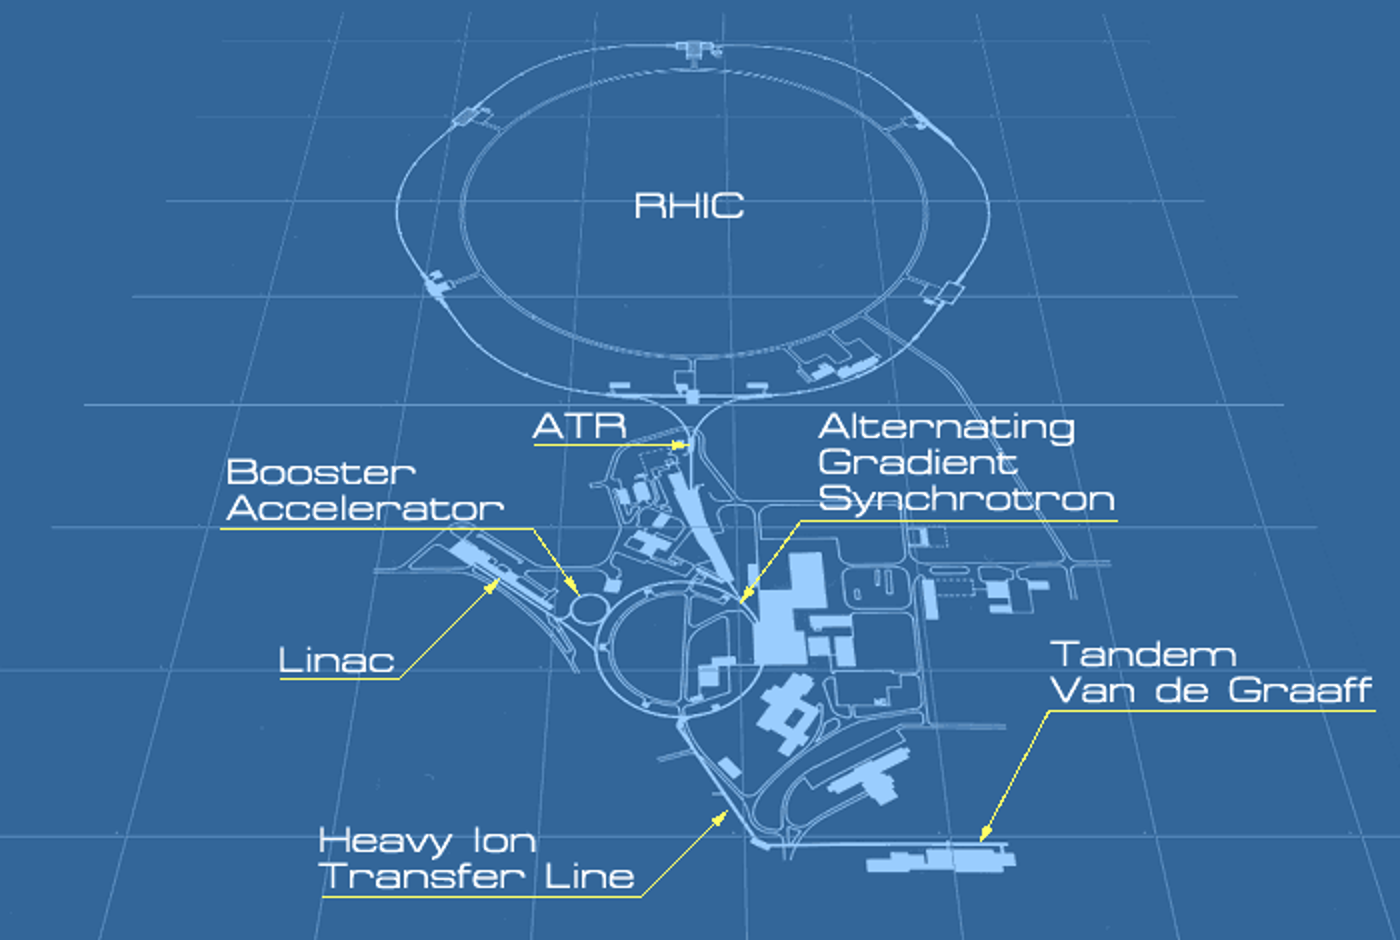
\includegraphics[width=0.8\textwidth,clip]{figures/Chapter2/RHIC.png}
    \end{center}
    \caption[相对论重离子对撞机(RHIC)综合装置示意图]{相对论重离子对撞机(RHIC)综合装置示意图}
    \label{fig:RHIC}
\end{figure}

金离子由脉冲溅射离子源(Pulser Sputter Ion Source)产生,带负电荷的金离子在串列范德格拉夫加速器(Tandem Van de Graaff)中被剥离一部分电子,变成电荷量为+32的金离子并被加速到 1MeV/$\mu$。之后电荷量为+32的金离子经过传输线被输送到增强器(Booster Synchrotron)中,在增强器中金离子被加速到 95 MeV/$\mu$ 并且外层电子被进一步剥离变成电荷量为+77的金离子并被注入到交变梯度同步加速器(Alternating Gradient Synchrotron, AGS)当中进行进一步的加速。电荷量为+77的金离子在交变梯度同步加速器被加速达到RHIC的注入能量 10.8 MeV/$\mu$后被送入AGS至RHIC的束流转移线(AGS-to-RHIC Beam Transfer Line)。金离子在束流转移线当中被剥离掉最后的电子成为电荷量为+79的离子后注入到RHIC当中,最后在RHIC中加速到对撞所需要的束流能量。
\section{RHIC上的螺线管径迹探测器——STAR}
RHIC上的螺线管径迹探测器(Solenoidal Tracker at RHIC,STAR)是坐落于RHIC 6点钟方向的大型粒子物理实验装置。在设计之初STAR就被赋予了丰富的物理目标,用以研究相对论重离子对撞产生的介质以及核子结构。整个探测器由多个子探测器组成,可以在高带电粒子多重数(RefMult)的环境下对末态粒子的径迹、动量、种类、能量等信息进行测量。在中心快度区间 ($|\eta| < 1 $),STAR具有全方位角 ($ 0 < \phi < 2\pi$)的接收度。STAR的核心径迹探测器为时间投影室(Time Projection Chamber, TPC),其可以对带电粒子的径迹进行测量并且通过电离能损信息($ \langle dE/dx \rangle $ )来进行粒子鉴别。

本文中的工作主要涉及以下子探测器:时间投影室,飞行时间探测器(Time of Flight, TOF),顶点位置探测器(Vertex Position Detector, VPD)以及STAR前向升级当中的小气隙板室(small-strip Tiny Gap Chamber, sTGC)。接下来的几个小节中将会对这些探测器进行简要的介绍。

\subsection{时间投影室}
\label{chap:TPC}
时间投影室是STAR最为核心的探测器也是STAR主要的径迹探测器。它可以提供穿过时间投影室的带电粒子的径迹和电离能损信息,并且通过这些信息计算径迹对应的粒子的动量和进行粒子鉴别。

其结构如图 \ref{fig:TPC} 所示。整个时间投影室为长4.2米,半径为2米的筒状结构。外部被一个大型螺线管磁铁环绕,用以提供沿着束流方向的匀强磁场。桶部为工作气体为P10 (10\%甲烷与90\%的混合气体)的漂移区,漂移区中心为内场膜,可以提供约为 135V/cm 的匀强电场。在端盖处为基于多丝正比室(Multi-Wire Proportional Chambers, MWPC)的读出系统。整个端盖处被分为了12 $\times$ 2个扇区,每个扇区为一个独立的多丝正比室。一个扇区的结构如图\ref{fig:MWPC}所示
\begin{figure}[htb]
    \begin{center}
    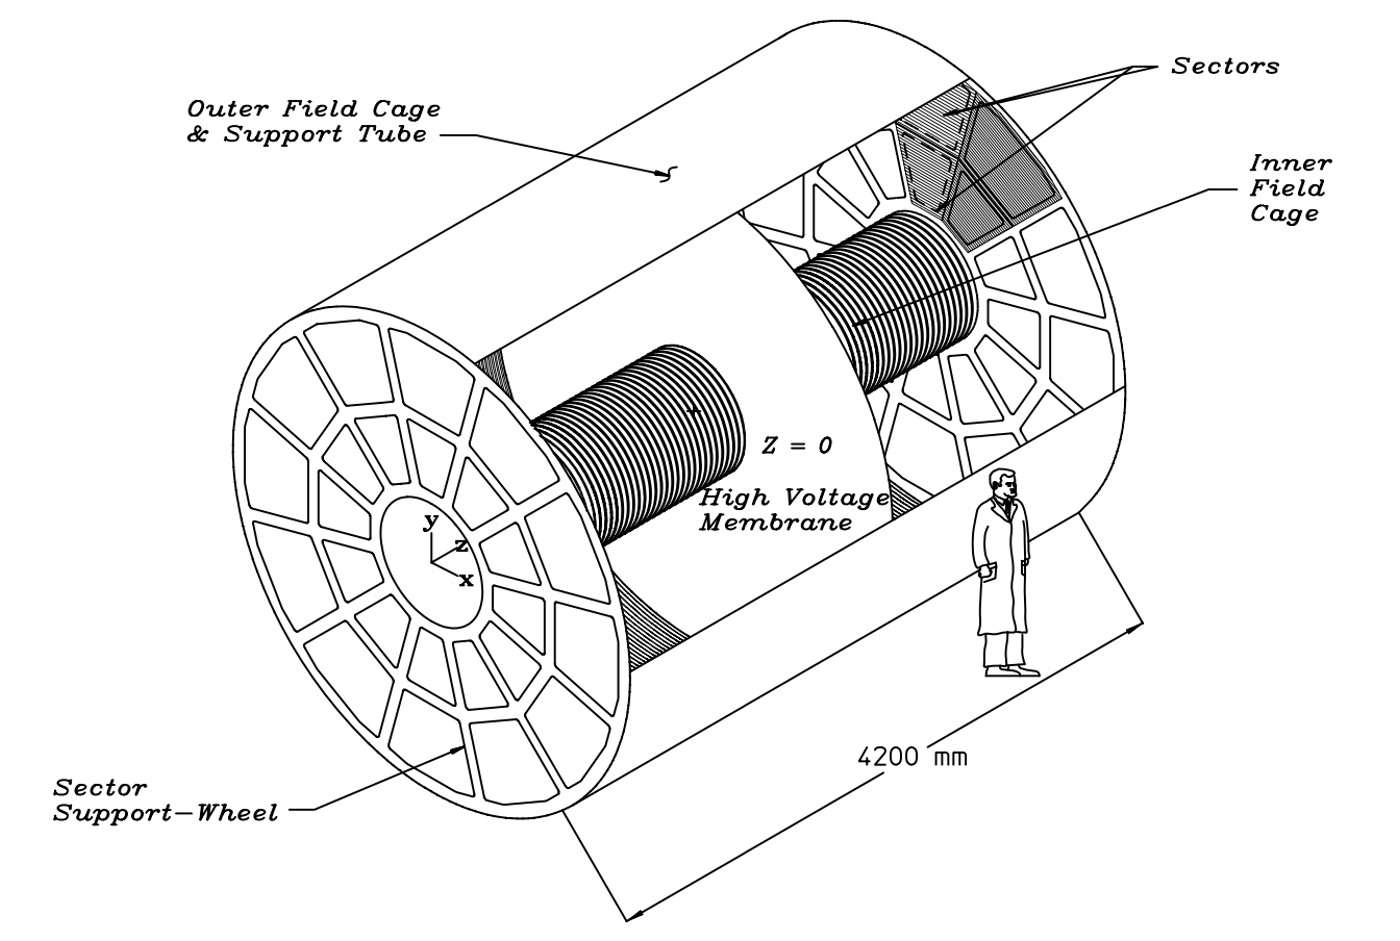
\includegraphics[width=0.75\textwidth,clip]{figures/Chapter2/TPC.png}
    \end{center}
    \caption[TPC结构示意图]{TPC结构示意图}
    \label{fig:TPC}
\end{figure}

图 \ref{fig:TPC_sector} 为时间投影室在2019年之前的扇区示意图,其中pad板排列密集的扇区为外扇区(outer sector),pad板排列稀疏的扇区为内扇区(inner sector)。从图中可以看到,内扇区的pad板排列明显稀疏于外扇区,粒子在穿过内扇区时最多留下13个击中(Hit)的信息用以径迹重建,这导致时间投影室在 $\eta$ 相对较大的范围的接收度变差。STAR于2019年进行了TPC内扇区(inner TPC, iTPC)的升级,对全部的内扇区进行替换升级,升级后的内扇区结构示意图见图 \ref{fig:iTPC} 。可以看到升级之后的内扇区的pad板密度明显增加。内扇区升级提高了整个时间投影室在大的$\eta$区间接收度、提升了时间投影室的径迹重建和粒子鉴别的能力并且使得时间投影室对低横动量的粒子的测量能力得到了进一步的提升。

\begin{figure}[htb]
    \centering
    \begin{subfigure}[b]{0.47\textwidth}
        \centering
        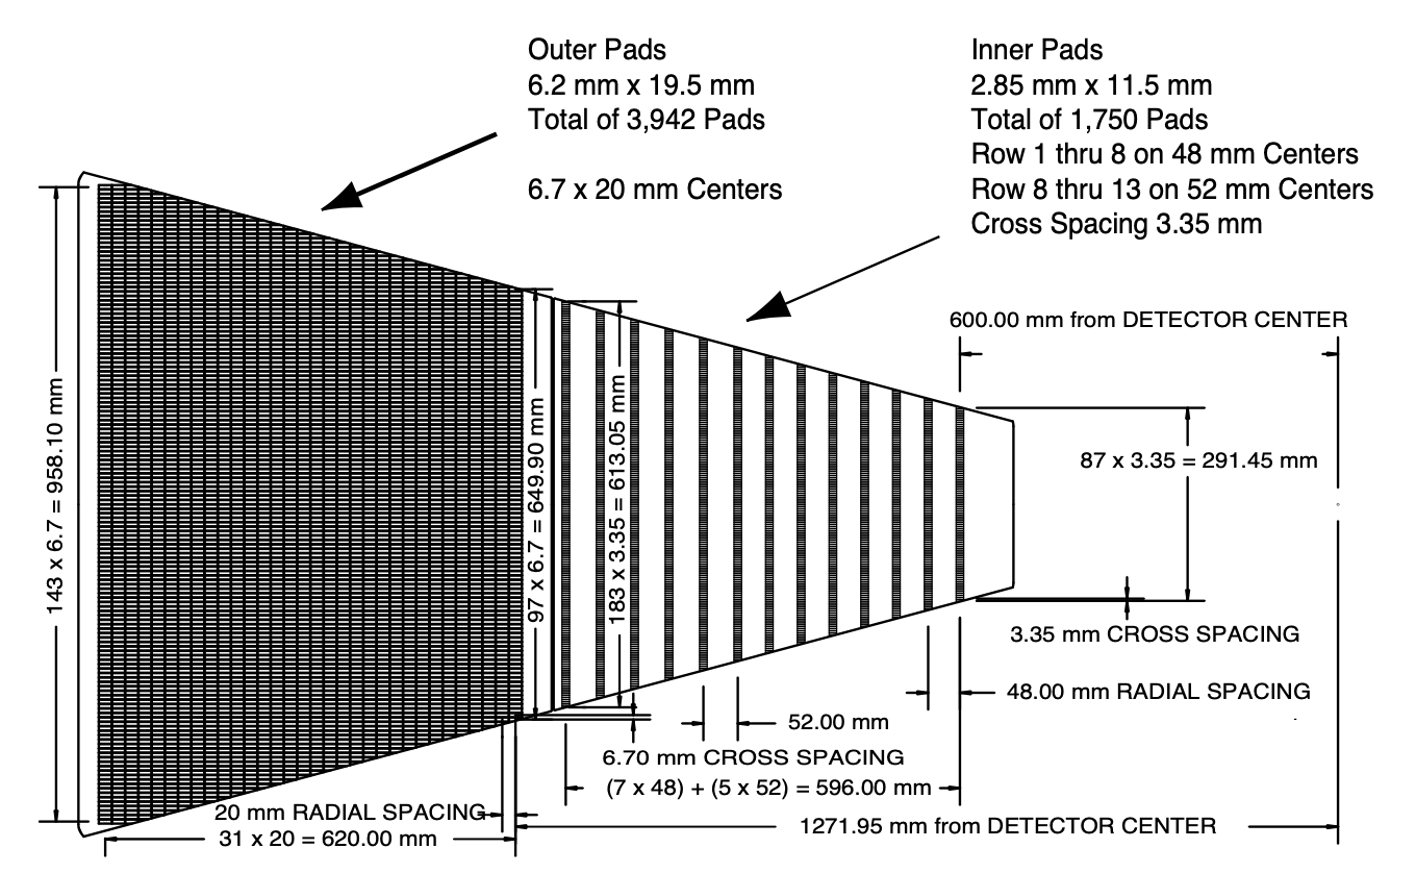
\includegraphics[width=\textwidth,clip]{figures/Chapter2/MWPC.png}
        \caption{}
        \label{fig:TPC_sector}
    \end{subfigure}
    \hfill
    \begin{subfigure}[b]{0.47\textwidth}
        \centering
        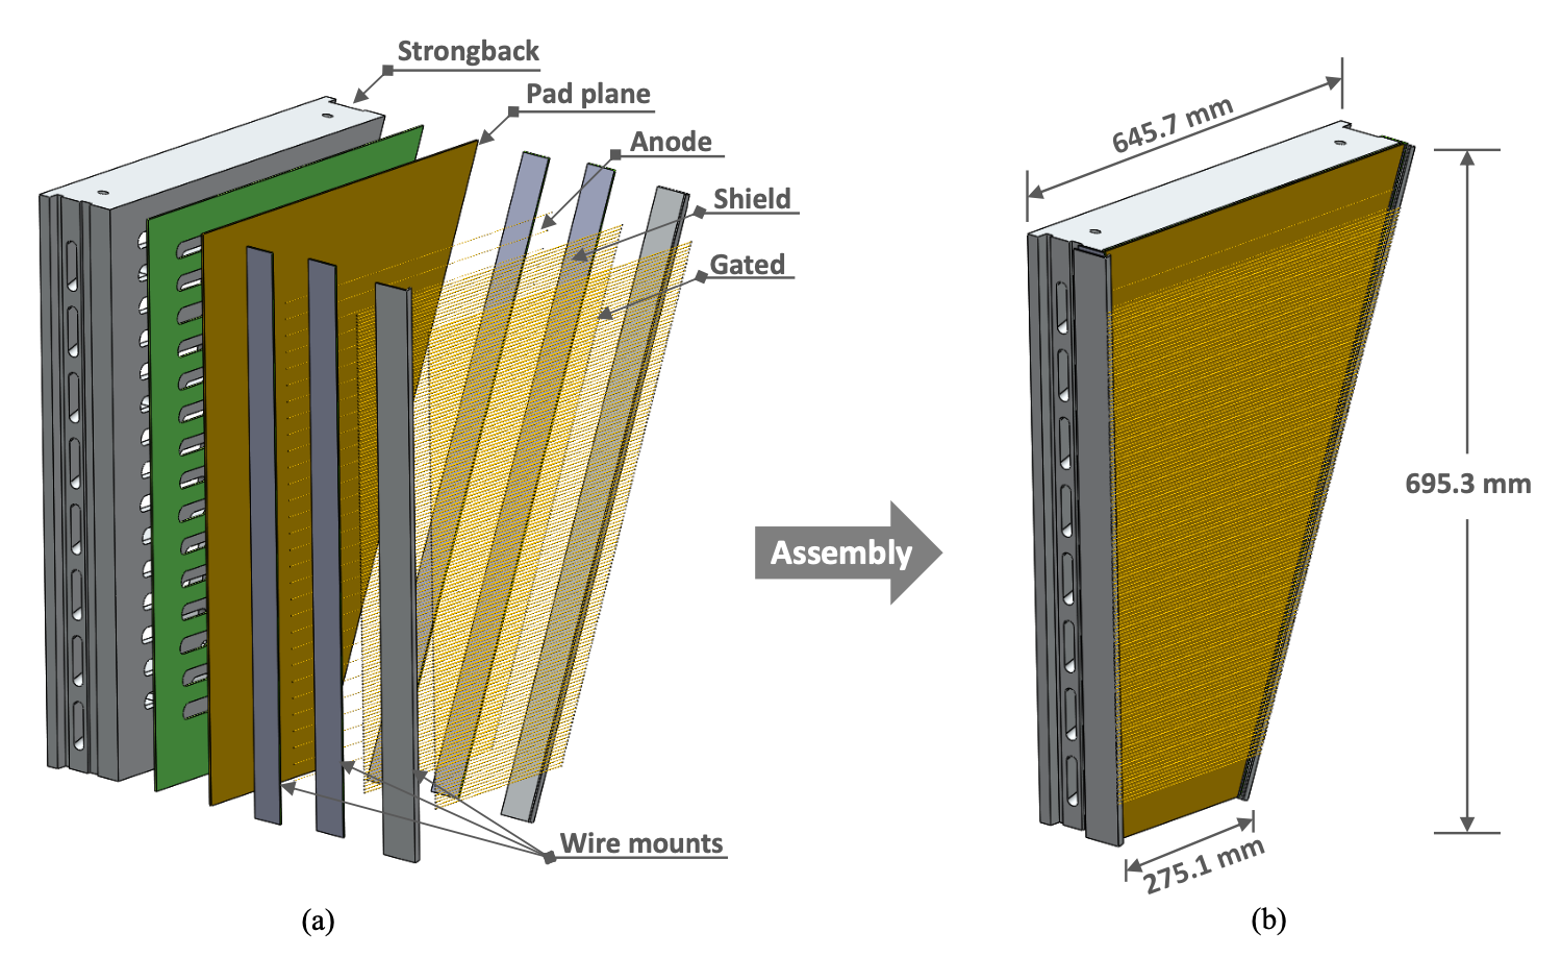
\includegraphics[width=\textwidth,clip]{figures/Chapter2/iTPC.png}
        \caption{}
        \label{fig:iTPC}
    \end{subfigure}
       \caption[TPC扇区示意图与iTPC升级后结构示意图]{图(a)为时间投影室升级之前一个扇区示意图,其中pad板排列密集的扇区为外扇区,pad板排列稀疏的扇区为内扇区。图(b)为升级后的内扇区结构示意图}
       \label{fig:MWPC}
\end{figure}

当带电粒子穿过时间投影室的时候,带电粒子会在匀强磁场的作用下发生偏转并且在漂移区的工作气体中电离产生原初电子-离子对,其中的电子在匀强电场的作用下向端盖处由多丝正比室组成的读出端漂移。因为P10气体的性质,电子在较低的电压下有着比较高的漂移速度。同时又因为时间投影室在漂移速度曲线的峰值附近工作,所以整个漂移速度受到气压和温度的影响较小,可以保持一个比较稳定的漂移速度。在STAR的取数过程中,也会每隔四个小时采集一个laser run来对时间投影室的漂移速度进行校正。
整个漂移过程中,电子束团(Cluster)的横向扩散约为 $\sigma_{T} = 3.3mm$ (漂移距离210cm),纵向(沿着漂移方向)扩散为$\sigma_{L} = 5.2mm$。对时间投影室来说,电子束团在横向和纵向的扩散会直接影响读出端丝室的设计。
当电子漂移到时间投影室的端盖处,电子会在通上高压的阳极丝附近发生雪崩过程,同时在阴极的pad板平面上产生感应信号,此感应信号被电子学采集之后通过电荷重心法可以确定出一个击中(Hit)的 X,Y 位置。因为整个漂移过程中漂移速度是稳定的,所以Z方向上的位置由漂移时间来决定。图\ref{fig:HowTPCWrok}展示了粒子在时间投影室中产生信号并被收集的过程。

\begin{figure}[htb]
    \begin{center}
    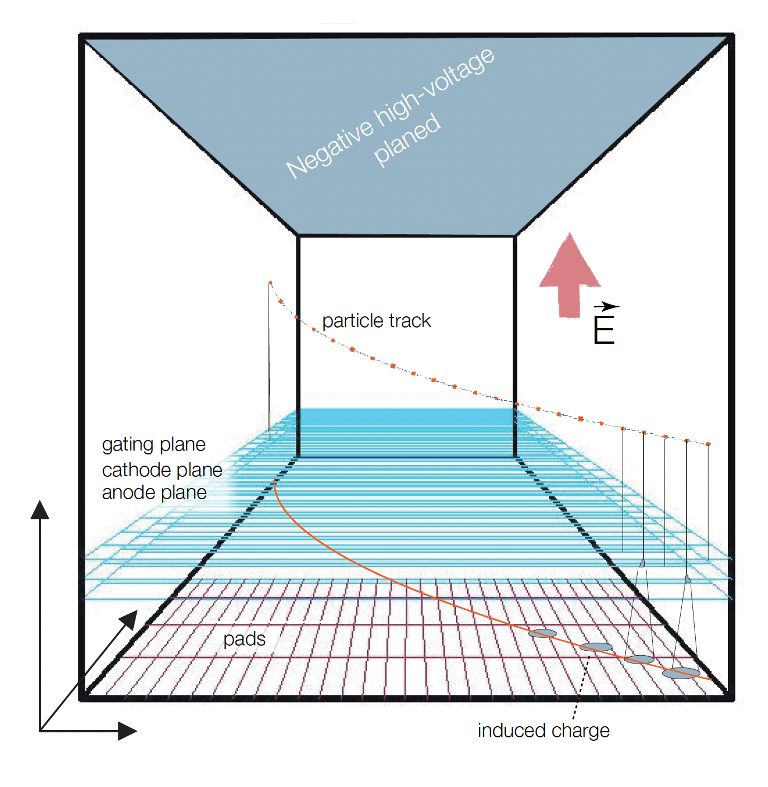
\includegraphics[width=0.75\textwidth,clip]{figures/Chapter2/HowTPCWork.png}
    \end{center}
    \caption[时间投影室工作原理示意图]{时间投影室工作原理示意图,展示了粒子在TPC中电离后产生的原初电离电子经由读出端丝室放大后在pad平面上产生感应信号的过程}
    \label{fig:HowTPCWrok}
\end{figure}

以上就是在时间投影室中带电粒子发生一次电离并且通过读出端收集到信号进行击中重建的大致过程。在一次对撞发生时会产生大量的末态的带电粒子,这些粒子在穿过漂移区的时候会发生多次电离,在读出端留下大量的击中信息。在收集到这些信号之后,需要通过算法将这些击中重建成径迹(Track)。

在时间投影室端盖处作为信号收集系统的多丝正比室工作在正比区,所以读出系统采集到的信号幅度大小和带电粒子在时间投影室中电离损失的能量成正比。当粒子在气体中电离时,其平均电离能损$ \langle dE/dx \rangle $可以通过Bethe-Bloch公式计算得到,公式如下:
\begin{equation}
    -\frac{dE}{dx} = 4\pi N_A r_c^2 m_e c^2 z^2\frac{Z}{A}\frac{1}{\beta} \bigg[ ln\frac{2 m_e c^2 \beta^2 \gamma^2 }{I} - \beta^2 - \frac{\delta}{2} \bigg ]
    \label{eq:BB}
\end{equation}

其中z为入射粒子电荷,Z为介质的原子序数,A为介质的原子量,$M_e$为电子质量,$r_c$是电子经典半径,$N_A$是阿伏伽德罗常数,I为介质的平均激发能,$\beta = v/c$为带电粒子的速度,$\delta$为描述入射的相对论性粒子的横向电场被原子电子电荷密度屏蔽程度的参数。需要注意的是,上式适用于入射粒子质量远大于电子质量的情形。当入射粒子为电子时,Bethe-Bloch公式可以近似为:
\begin{equation}
    -\frac{dE}{dx} = 4\pi N_A r_c^2 m_e c^2 \frac{Z}{A}\frac{1}{\beta} \bigg[ \frac{1}{2}ln\frac{m_e c^2 \gamma }{2I} - \beta^2 - \frac{\delta^*}{2} \bigg ]
\end{equation}
其中$\delta^*$与式 \ref{eq:BB} 中的$\delta$略有不同。图 \ref{fig:dEdx}为不同粒子在时间投影室中电离能损随动量变化的示意图,可以看到在相同的动量的时候不同粒子有着不同的电离能损,时间投影室就可以通过测量径迹的平均电离能损$ \langle dE/dx \rangle $的方式来进行粒子鉴别。同时可以看到在动量较高的区间电子和 $\mu$子,$\pi$介子的电离能损无法较好的分辨。我们需要额外的信息来帮助我们进行粒子鉴别,例如速度信息。粒子速度的测量将在下一小节中进行介绍

\begin{figure}[htb]
    \begin{center}
    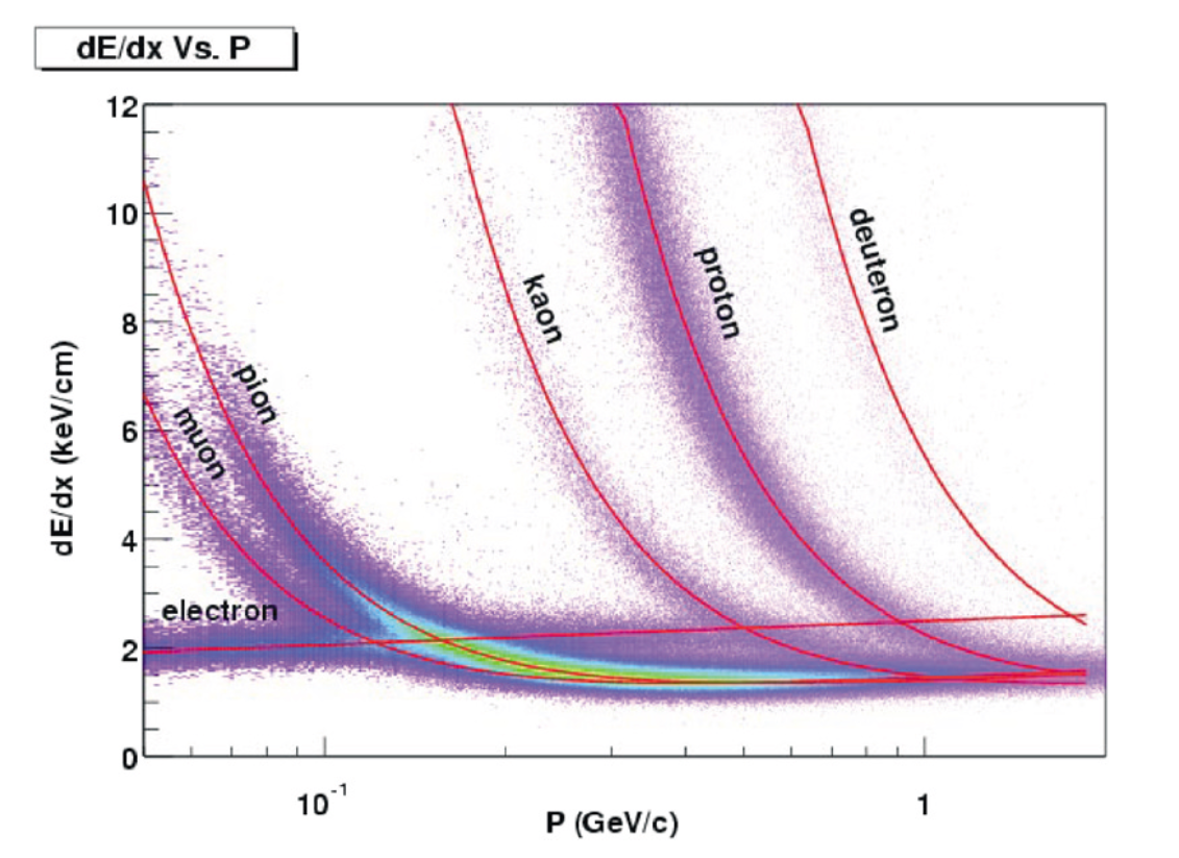
\includegraphics[width=0.75\textwidth,clip]{figures/Chapter2/dEdx.png}
    \end{center}
    \caption[粒子在时间投影室中的电离能损]{不同种类粒子在时间投影室中电离能损随着动量变化示意图。本图中数据在磁场为0.25T的环境下测量}
    \label{fig:dEdx}
\end{figure}

\subsection{飞行时间探测器}

如上小节中所讨论,在动量相对较高的区间我们需要额外的信息来帮助进行粒子鉴别。飞行时间探测器(Time of Flight, ToF)被设计用来测量粒子的飞行速度从而进行粒子鉴别。这就对TOF的性能提出了如下要求:
\begin{itemize}
    \item 时间分辨率小于100ps, 对于停止时间(Stop time)的测量,时间分辨率应小于80ps。
    \item 每个通道的响应时间快,从而可以在在高粒子多重数的环境下工作
    \item 可以在STAR的磁场环境(0.5T)下稳定工作
    \item 成本相对较低,可以覆盖较大的范围从而与TPC中的径迹进行配对,空间接收度应与TPC类似。
\end{itemize}

基于这这些需求,多气隙电阻板室(Multi-gap Resistive Plate Chamber, MRPC)被用来作为TOF的终止时间测量探测器,起始时间由顶点位置探测器(Vertex Position Detector, VPD)给出。多气隙电阻板室首先被应用在ALICE实验上的时间飞行探测器当中,有着很高的时间分辨率且可以在高粒子多重数、强磁场的环境下工作。图 \ref{fig:MRPC} 为STAR中多气隙电阻板室的结构示意图。
\begin{figure}[htb]
    \begin{center}
    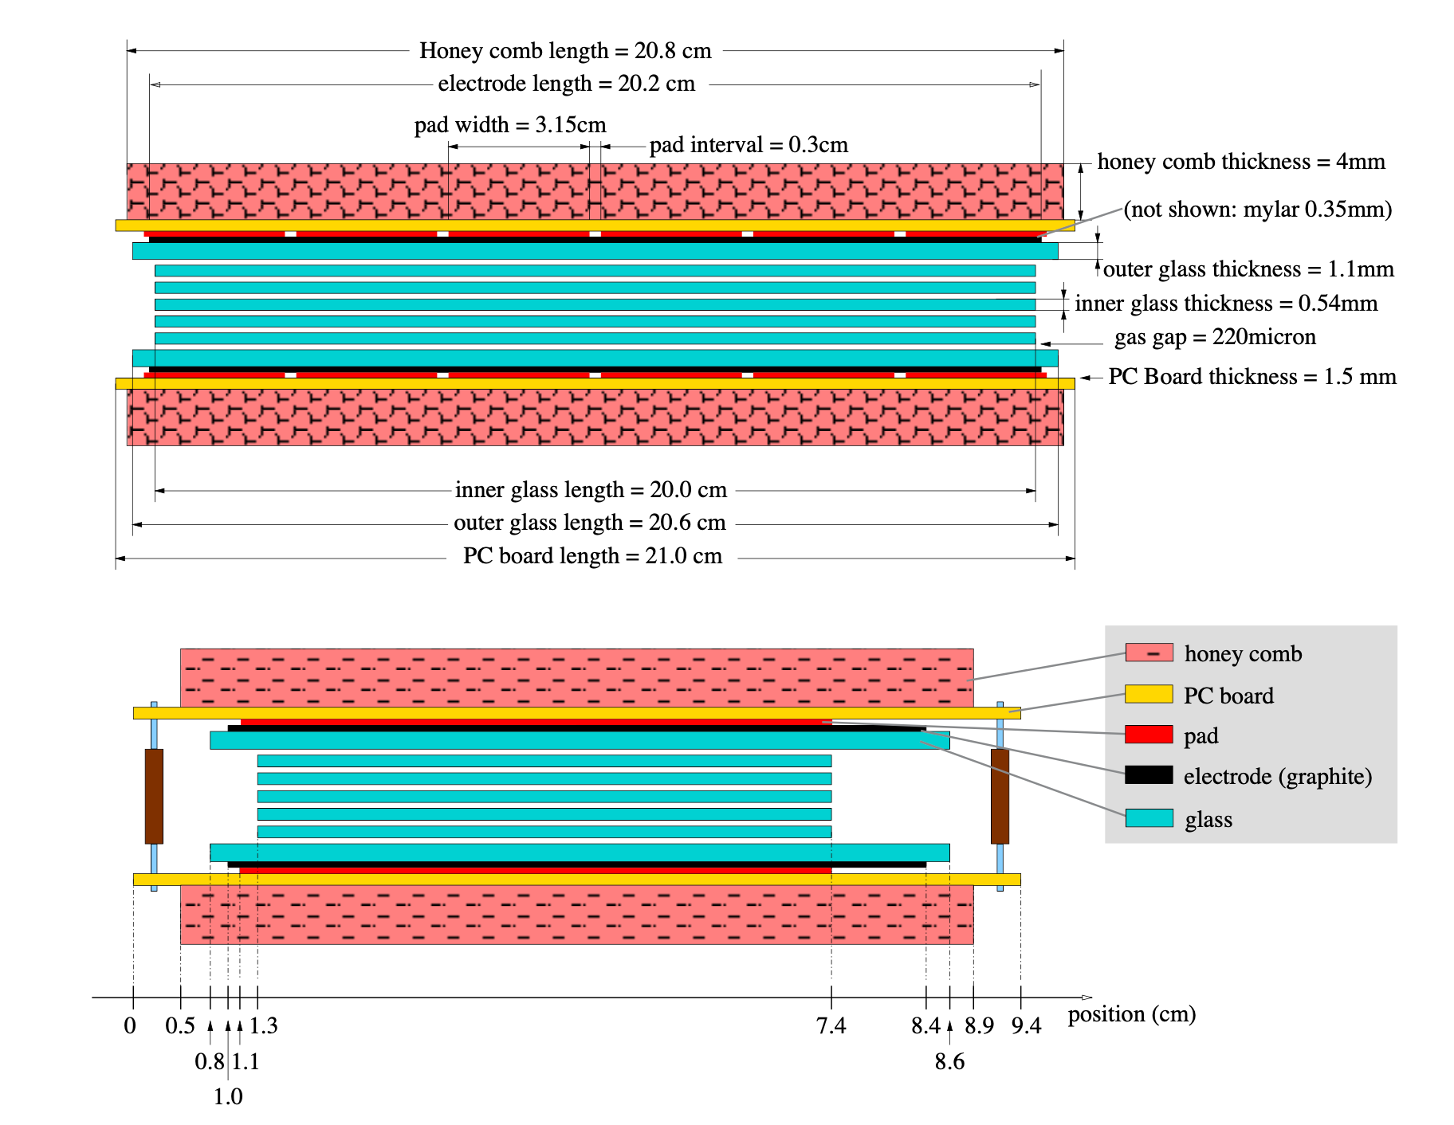
\includegraphics[width=0.7\textwidth,clip]{figures/Chapter2/MRPC.png}
    \end{center}
    \caption[MRPC结构示意图]{STAR上MRPC的测试图,上图为沿长边方向,下图为沿短边方向}
    \label{fig:MRPC}
\end{figure}
如图所示,在两个电极之间插入了5块阻性玻璃板,电极之间加有高压,可以在阻性板和阻性板之间的气隙之间产生高压。当带电粒子穿过整个室的时候可以在每个气隙处发生独立的雪崩过程。对于整个室而言,读出端所得到的感应信号相当于多个间隙内雪崩的“瞬时”叠加,因此可以获得一个相对较大的信号。多气隙电阻板室相对于传统的的阻性板室(Resistive Plate Chamber, RPC)计数率可以得到很大的提高。每个多气隙电阻板室具有6个 6.1 $\times$ 3.4cm 的读出pad,这使得飞行时间探测器的读出有着相对较好的读出粒度,使飞行时间探测器上的击中可以与时间投影室中的径迹进行配对。飞行时间探测器中的多气隙电阻板室的接收度和时间投影室类似,也有着全方位角($ 0 < \phi < 2\pi$)和中心快度区间($ |\eta| < 0.9 $)的接收度。

结合多气隙电阻板室测得的终止时间和顶点位置探测器测得的起始时间可以得到径迹的飞行时间,再利用时间投影室测量得到的径迹长度信息可以计算得到粒子的飞行速度用以进行粒子鉴别,图 \ref{fig:TOFPerformance} 展示了TOF测量的 $1/\beta$ 随动量变化的分布以及添加 $1/\beta$ 判选条件后的电离能损分布。可以看到,在额外添加$|1-1/\beta| < 0.03$的判选条件时,电子的电离能损可以很好的与其他粒子区分开来。整个STAR探测器的粒子鉴别能力在添加径迹的速度信息后得到了很好的提升。

\begin{figure}[htb]
    \centering
    \begin{subfigure}[b]{0.47\textwidth}
        \centering
        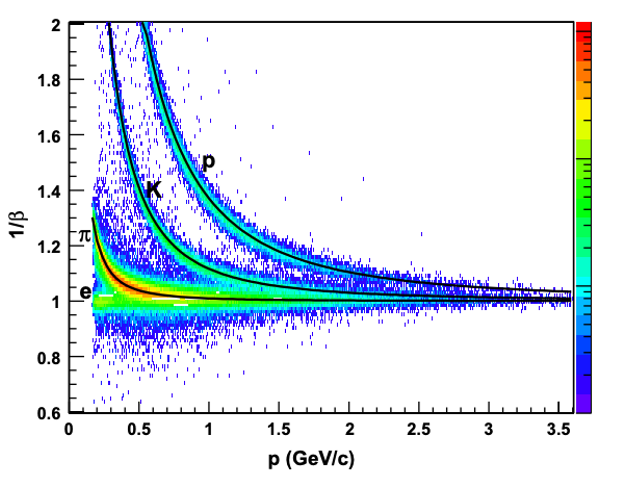
\includegraphics[width=0.9\textwidth,clip]{figures/Chapter2/BetaDistribution.png}
        \caption{}
        \label{fig:BetaDis}
    \end{subfigure}
    \hfill
    \begin{subfigure}[b]{0.47\textwidth}
        \centering
        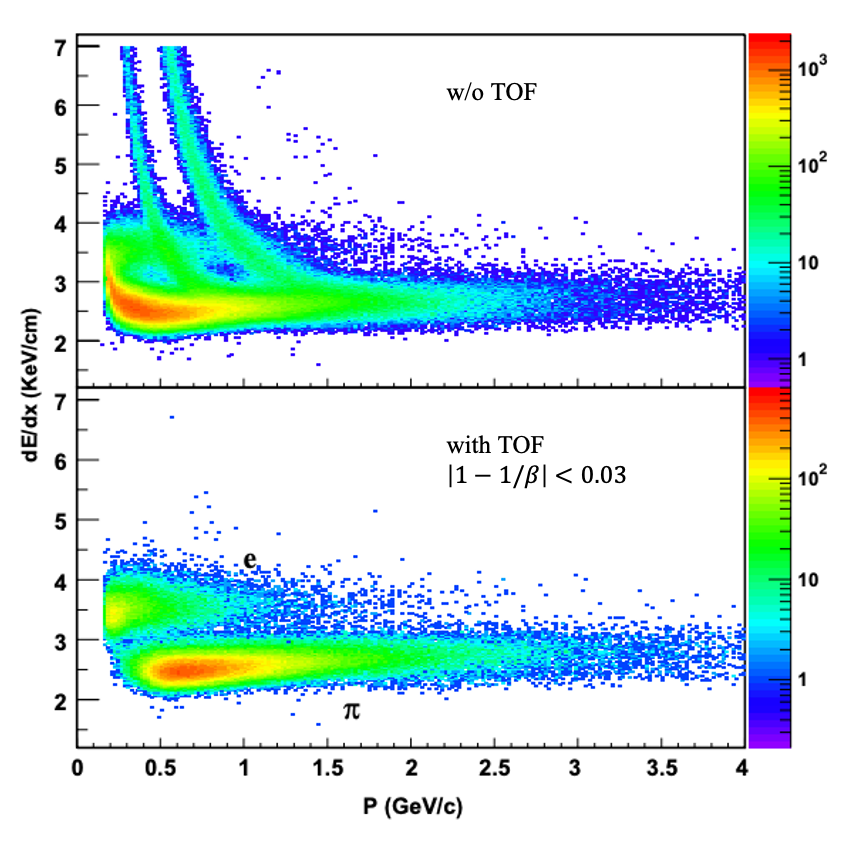
\includegraphics[width=0.9\textwidth,clip]{figures/Chapter2/dEdxwithTOF.png}
        \caption{}
        \label{fig:dEdxwithTOF}
    \end{subfigure}
       \caption[飞行时间探测器粒子鉴别表现]{图(a)粒子的$1/\beta$分布随着动量变化的示意图。图(b)为电离能损(dE/dx)随着动量变化的分布。上半部分为仅用时间投影室测量,不添加额外的关于$\beta$的判选条件的电离能损分布。下半部分为在上半部分基础上额外添加 $|1-1/\beta| < 0.03$的判选条件时的电离能损分布}
       \label{fig:TOFPerformance}
\end{figure}
  



